\documentclass[twoside, a4paper]{article}
\usepackage{fontenc}
\usepackage{inputenc}
\usepackage[english,russian]{babel}
\usepackage{amsmath}
\DeclareMathOperator{\sech}{sech}
\usepackage{amsfonts}
\usepackage{amssymb}
\usepackage{makeidx}
\usepackage{multirow}
\usepackage{lipsum}
\usepackage{fancyhdr} 
\usepackage{graphicx}
\graphicspath{ {./pictures/} }
\usepackage[
    top=30mm,
    bottom=20mm,
    left=20mm,
    right=20mm
]{geometry}
\pagestyle{fancy} 
\fancyhf{}
\fancyhead[CE]{4.8 Гамильтоновы система с двумя степенями свободы \ldots} 
\fancyhead[CO]{Глава 4}
\fancyhead[R]{\thepage}
\setcounter{page}{270}
\begin{document}
\newcounter{taskc}
\renewcommand{\thetaskc}{4.8.\arabic{taskc}}
\newcommand{\task}[1]{\par\vspace{0.4cm}\refstepcounter{taskc} \texttt{Упражнение \thetaskc} {\small#1}\vspace{0.4cm}}
\task{
Рассмотрите <<нелинейный гармонический>> осциллятор с гамильтонианом\\ $H=\frac13(p_1^2+q_1^2)^{3/2}+\frac12(p_2^2+q_2^2)$. Покажите, что редуцированную систему можно записать в виде 
$$q_1'=p_1\sqrt{p_1^2+q_1^2},$$
$$p_1=-q_1]\sqrt{p_1^2+q_1^2},$$
откуда сделайте вывод, что отображание Пуанкаре имеет два плотных множества замкнутых кривых, одно из которых заполнено периодическими орбитами, другое --- плотными орбитами.
}\label{red_sys}
\task{
Проведите редукцию модели <<маятник-осциллятор>> с гамильтонианом
$$H(q_1,p_1,q_2,p_2)=\frac{p_1^2}{2}+(1-\cos q_1)+\frac{p_2^2+\omega_2^2g_2^2}{2}$$
и обсудите соответствующее отображение Пуанкаре. (Мы вернёмся к этому примеру позже в данном разделе.)
}\label{osc}

Примеры, которые мы обсуждали до сих пор, являются \textit{вполне интегрируемыми} в том смысле, что имеется \textit{две независимые} функции (одна из которых $H$), остающиеся инвариантными относительно потока, определяемого уранвениями Гамильтона. Для первого из примеров в качестве второй функции можно взять действие для второго из осцилляторов
$$I=(p_2^2+\omega_2^2q_2^2)/2\omega_2,$$
при этом решения лежат на двумерных торах, представляющих собой пересечения поверхностей
\renewcommand{\theequation}{4.8.\arabic{equation}}
\setcounter{equation}{17}
\begin{equation}
H = h^0,\text{~~} I=I^0
\end{equation}

Аналогично можно рассмотреть примеры из упражнений \ref{red_sys}-\ref{osc} Однако, как понимали Пуанкаре и Биркгоф, очень немногие системы с двумя степенями свободы обладают двумя независимыми интегралами, и классическая теория Гамильтона-Якоби, связанная с отысканием такт интегралов, в болыиинстве случаев не срабатывает. Более того, попытки приближенного вычисления второго интеграла методами усреднения или теории возмущений, а также путем вычисления нормальной формы в такт случаях не приводят к успеху. Мы отсылаем читателя к книге Lichtenberg, Lieberman [1982], где обсуждаются эти методы, огранияиваясь здесь демонстрацией того, как метод Мельникова в сочетании с редукцией может быть использован для доказательства несуществования второго (аналитического) интеграла движения в конкретных примерах. При обсуждении этого метода мы сделаем также ряд общих наблюдений о свойствах двумерного отображения Пуанкаре $P_{h^0}^{\Theta_0}$ редуцированной системы. В дальнейшем мы будем опускать индексы $h^0$, $\Theta_0$ и  писать $P_{h^0}^{\Theta_0}=P_\varepsilon$ или $P_0$, где индексы свидетельствуют о наличии или отсутствии возмущения $\varepsilon H^1$ в нижеследующем уравнении (\ref{eq:label1}).
Вначале заметим, что $P$ --- сохраняющий площадь диффеоморфизм, так
как
%$$-\frac{\partial^2L}{\partial q\partial p}$$
\begin{equation}
DP=e^{2\pi Df} , \text{~~}  Df=
\left[\begin{array}{cc}
-\frac{\partial^2L}{\partial q\partial p} & -\frac{\partial^2L}{\partial p^2} \\
-\frac{\partial^2L}{\partial q\partial p} & -\frac{\partial^2L}{\partial p^2}
\end{array}\right]
\end{equation}
и след матрицы $Df$ тождественно равен нулю. (Сохранение объёма, в силу теоремы Лиувилля, проявляется здесь в сохранении площади при отображении $P$.)
Предположим далее, что наш гамильтониан является (малым) возму- щением $H^\varepsilon$ некоторого интегрируемого гамильтониана $H^0$ . Возьмем для простоты систему вида
\begin{equation}
H^\varepsilon (q,p,\Theta,I) = F(q,p)+G(I)+\varepsilon H^1(q,p,\Theta, I),
\label{eq:label1}
\end{equation}

где функция $ H^1 $ имеет по $\Theta$ период $ 2\pi $, а невозмущённая система $H^0(q,p,\Theta,I)=F(q,p)+G(I)$ непосредственно распадается на две независимые системы с интегралами $F$ и $G$ (или, что равносильно, $H^0$ и $I$. Как и ранее, сделаем предпололжение о невырожденности
\newcommand*{\defeq}{\stackrel{\text{def}}{=}}
\begin{equation}
\Omega(I) \defeq \frac{\partial G}{\partial I} \left(=\frac{\partial H^0}{\partial I}\right) \neq 0
\end{equation}
конкретнее, $\Omega>0$ при $I>0$. Отсюда следует, что для малых $\varepsilon$ уравнение $H^\varepsilon = F+G+\varepsilon H^1=h$ разрешимо относительно I как и ранее. Однако наличие здесь малого параметра $\varepsilon$ позволяет нам вычислить обратую функцию $L$ в уравнении (4.8.7) %оно не в моей главе
явно в виде рядов по степеням $\varepsilon$. Мы имеем 
\begin{equation}
\text{~}\begin{aligned}
&I=L^\varepsilon (q,p,\Theta;h) = L^0(q,p;h)+\varepsilon L^1(q,p,\Theta;h) + O(\varepsilon^2),\\
&l^0=G^{-1}(h-F(q,p)),\\
&L^1=-\frac{H^1(q,p,\Theta,L^0(q,p;h))}{\Omega(L^0(q,p;h))}
\end{aligned}
\label{eq:label2}
\end{equation}
\task{проверьте соотношения (\ref{eq:label2})}

В силу (\ref{eq:label2}) редуцированная гамильтонова система принимает вид
\begin{equation}
\text{~}\begin{aligned}
&q'=-\frac{\partial L^0}{\partial p}(q,p;h)-\varepsilon\frac{\partial L^1}{\partial p}(q,p,\Theta;h)+O(\varepsilon^2),\\
&p'=\frac{\partial L^0}{\partial q}(q,p;h)+\varepsilon\frac{\partial L^1}{\partial q}(q,p,\Theta;h)+O(\varepsilon^2),\\
\end{aligned}
\label{eq:label3}
\end{equation}
Поскольку $H^1$ является $2\pi$-периодической функцией $\Theta$, такова же и $L^1$, так что система (\ref{eq:label3}) относится именно к тому типу, который изучался в предыдущем разделе при помощи метода Мельникова.

В частности, допустим (как выше), что некоторая (компактная) область фазовой плоскости для системы $F(q,p)$ заполнена периодическими орбитами, периоды которых монотонно изменяются при изменении энергии $F$. Каждая такая орбита является множеством уровня для $F:F(q,p)=h^\alpha$, следовательно, если общая энергия $h$ больше,чем $h^\alpha$, невозмущённая $(\varepsilon=0)$ автономная система (\ref{eq:label3}) имеет соответстсвующую замкнутую орбиту, описываемую формулой
\begin{equation}
L^0(p,q,h)=G^(-1)(h-h^\alpha)\defeq l^\alpha
\end{equation}
\renewcommand{\thefigure}{4.8.\arabic{figure}}
Кроме того, период этой орбиты $T^\alpha$ монотонно изменяется при измении $l^\alpha$
\begin{figure}[h]
\centering
\includegraphics[width=0.4\textwidth]{Poincarе_map}
\caption{Невозмущённое отображение Пуанкаре $P_0$ для \ref{eq:label3}}
\label{fig:pic1}
\end{figure}

Далее, отображение Пуанкаре $P^0$, ассоциированное с (\ref{eq:label3}) при $\varepsilon = 0$, является просто отображеним вдоль потока за время $2\pi$. Следовательно, оно обладает непрерывным семейством инвариантных замкнутых кривых, заполненных $m$-периодическими точками в случае, когда $T^\alpha = 2\pi m/n, m,n \in \mathbb{Z}$, или плотными орбитами, если отношение $T^\alpha / 2^\pi$ иррационально, см. рисунок \ref{fig:pic1} (ср. упражнение 4.8.1). Положим для простоты, что $T^\alpha$ возрастает при возрастании $l^\alpha$, так что среднее значение угла, на который поворачиваются точки под действием $P_0$, убывает по мере удаления инвариантных кривых от начала, как показано на рисунке \ref{fig:pic1}.

Переходя от $(p,q)$ к некоторым переменным <<действие -угол>> $J,  \phi$, приведём невозмущённую систему к виду 
\begin{equation}
\text{~}\begin{aligned}
&\dot J = 0, \\
&\dot \phi = A(J),\\
\end{aligned}
\end{equation}
где $A(J) = 2\pi / T^\alpha$, и отображение Пуанкаре запишется так:
\begin{equation}
(J, \phi) \stackrel{P_0}{\longmapsto} (J, \phi + 2 \pi \Lambda (J)).
\label{eq:e4826}
\end{equation} 

По предположению, величина $Lambda$ убывает с ростом $J$, поэтому $P_0$ является \emph{закручивающим отображением}. Возмущение $\varepsilon L^1$ изменит его следующим образом: 
\begin{equation}
(J, \phi) \stackrel{P_\varepsilon}{\longmapsto} (J + \varepsilon f(J, \phi, \varepsilon), \phi + 2 \pi \Lambda (J) + \varepsilon g(J, \phi, \varepsilon))
\label{eq:e4827}
\end{equation} 
где $f$ и $g$ --- ограниченные $2\pi$-периодические по $\phi$ функции, причём $P_\varepsilon$ по-прежнему сохраняет площадь.

Прежде, чем представить метод определения свойств преобразования $P_\varepsilon$, приведём некоторые результаты, касающиеся возмущений, сохраняющих площадь отображений, подобных $P_0$. Более полнуая информация содержится в Arnold, Avez [1968, особенно \S 19--21, 34], Moser [1973], Арнольд [1978]. Наиболее важным результатом является знаменитая теорема Колмогорова--Арнольда--Мозера (КАМ), утверждающая, что для достаточно малых $\varepsilon$ <<большинство>> замкнутых кривых $J=const$, инвариантных для $P_0$, сохраняется и для $P_\varepsilon$. Различные варианты этой теоремы были получены Колмогоровым [1954], Moser [1962], Арнольдом [1963a,b] и Rüssman [1970], а затем обобщены для систем с $n$ степенями свободы, для которых отображения Пуанкаре $(2n-2)$-мерны (см. Arnold, Avez [1968], Арнольд [1978])\footnote{Авторы не вполне точно излагают историю вопроса: на самом деле упомянутая основополагающая работа А. Н. Колмогорова посвящена сохранению инвариантных торов в многомерных гамильтоновых системах, близких к вполне интегрируемым. Представленная здесь теорема \ref{theorem1} принадлежит Арнольду и Мозеру --- \emph{Прим. перев.}}. Вместо того, чтобы приводить её наиболее общую формулировку, мы ограничимся контекстом обсуждаемого двумерного примера:
\newcounter{teoremc}
\renewcommand{\theteoremc}{4.8.\arabic{teoremc}}
\newcommand{\mytheorem}[2][]{\par\vspace{0.4cm}\refstepcounter{teoremc} \textbf{Теорема \theteoremc ~#1} {\emph{#2}}\vspace{0.4cm}}
%\textbb{Теорема 4.8.\theteoremc} {\italic#1}
\mytheorem[(КАМ)]{Если $A'(J)\neq 0$  и величина $\varepsilon$ достаточно мала, то возмущённое отображение $P_\varepsilon$ обладает множеством инвариантных замкнутых кривых, имеющих положительную меру Лебега $\mu (\varepsilon )$ и близких к исходному множеству $J = J^\alpha$. Более того, $\mu (\varepsilon)/\mu(J)\to 1$ при $\varepsilon \to 0$. Сохраняющиеся инвариантные замкнутые кривые заполнены плотными иррациональными орбитами}\label{theorem1}

Из этого результата следует, что в исходной гамильтоновой системе (\ref{eq:label1}) при малых $\varepsilon \neq 0$ сохраняется некоторое измеримое множество торов, несущих иррациональные потоки.

В терминах исходного невозмущённого гамильтониана
$$H^0(q,p,I)=F(q,p)+G(I)=F(J)+G(I)$$
условие невырожденности $A'(J) \neq 0$ выглядит так:
\begin{equation}
G''(I)(F''(J))^2+F''(J)(G'(I))^2 \neq 0
\label{eq:e4828}
\end{equation} 
для всех таких $I, J$, что $G(I)+F(J)=H$ (см. Арнольд [1978]).
\task{
Проверьте, что из условия (\ref{eq:e4828}) следует, что $\Lambda'(J) \neq 0$. Покажите, что если в невозмущённом гамильтониане $H^0(I,J)$ переменные не разделяются, то условие невырожденности имеет вид
\begin{equation}
\det
\left|\begin{array}{ccc}
H^0_{II} & H^0_{IJ} & H^0_{I}\\
H^0_{IJ} & H^0_{JJ} & H^0_{J}\\
H^0_{I} & H^0_{J} & 0
\end{array}\right|
\label{eq:e4829}
\end{equation}
Заметим, что условия (\ref{eq:e4828})--(\ref{eq:e4829}) выражают \emph{изоэнергетическую невырожденность}, они гарантируют, что отношение частот на невозмущённых инвариантных торах изменяется при переходе с одного тора на другой на каждом фиксированном уровне энергии (Арнольд [1978]).
}
\task{
Покажите, что отображение Пуанкаре для редуцированной системы из упражнения \ref{red_sys} можно представить в форме (\ref{eq:e4826}), где $\Lambda(J)=\sqrt{2J}$. Покажите также, что исходная система удовлетворяет условию \ref{eq:e4828}. (Подсказка: положите $q_2=\sqrt{2I}\sin \theta, p_2=\sqrt{2I} \cos \theta, q_1 = \sqrt{2J}\sin \phi, p_1 = \sqrt{2J} \cos \phi$.)
}

Общая картина (построенная, в основном, численно) такова: <<достаточно иррациональные>> замкнутые кривые сохраняются при малых $\varepsilon$ для \emph{произвольных} возмущений, однако с ростом $\varepsilon$ они исчезают одна за другой до тех пор, пока не останется ни одной замкнутой кривой, близкой к невозмущённой (хотя могут проявиться другие замкнутые кривые). Для уточнения понятия <<достаточно иррациональные>> приведём более конкретный результат, принадлежащий Мозеру:

\mytheorem[(теорема Мозера  {[1973]}, \S2).]{
 Рассмотрим малое сохраняющее площадь возмущение $P_\varepsilon$ некоторого сохраняющего площадь двумерного отображения $P_0$. Допустим, что функция $A(J)$ класса $C^r, г \geq 5$,причем $|А'(J)| \geq \nu > 0$ в некотором кольце $R = {(J, \phi) | a\leq J \leq b}$. Тогда существует такое число $\delta$, зависящее от $\varepsilon$ и $\Lambda(J)$, что если возмущение $P_\varepsilon$ удовлетворяет неравенству
\begin{equation}
\sup_{(J,\phi) \in R} \{ \|\varepsilon f \|_r + \|\varepsilon g\|_r\} < \nu \delta,
\end{equation} 
(здесь $\|\varepsilon f \|_r $ обозначает норму в $C^r$, т. е. $\sum_{k=0}^r |D^kf(J,\phi,\varepsilon)|)$, то $P_\varepsilon$ обладает в  $R$ инвариантной кривой $\Gamma_\varepsilon$ вида 
\begin{equation}
J = J^0 + U(\psi),\text{~} \phi = \phi + V(\psi),
\end{equation} 
где функции $U$ и $V$ класса $C^1$ и $2\pi$-периодичны, причём 
\begin{equation}
\|U\|_1 + \|V\|_1<\varepsilon
\end{equation} 
и $a<J^0<b$. Кроме того, индуцированное на этой кривой отображение $P_\varepsilon|\Gamma_\varepsilon$ задается формулой
\begin{equation}
\phi \to \phi + 2 \pi \lambda
\end{equation} 
где иррациональное число $\lambda$ удовлетворяет бесконечному множеству соотношений
\begin{equation}
\left|\lambda-\frac{n}{m}\right|\geq \gamma m^\alpha
\label{eq:e4834}
\end{equation} 
для некоторых $\gamma, \alpha > 0$ и всех натуральных $m,n$. Каждому выбору $\lambda$ в диапазоне $A(J)$ и удовлетворяющему условиям \ref{eq:e4834} отвечает некоторая такая инвариантная кривая.
}\label{moserTheorem}

Для обоих данных результатов центральным является условие, что $P_\varepsilon$ сохраняет площадь, так как если это отображение уменышает или увеличивает площади, инвариантные кривые могут не существовать\footnote{Как правило, не существуют. --- \emph{Прим. перев.}}. Мы вернемся к вопросу о числах вращения при обсуждении отображений окружности в разделе 6.2.

Сохранение множества инвариантных замкнутых кривых имеет важное следствие в вопросе об устойчивости движения исходной системы на каждом многообразии $H=h$, так как из его существования следует, что некоторые из исходных двумерных инвариантных торов $J=const$ сохраняются и выступают в роли ограничителей на трехмерных энергетических многообразиях, через которые не могут перейти решения. Возмущенные решения либо располагаются на этих торах, либо попадают в ловушку между парой таких торов и, следовательно, не могут уйти в фазовом пространстве сколь угодно далеко. Заметим, что хотя в системах с $n>3$ степенями свободы множества аналогичных $n$-торов также сохраняются, они уже не могут служить ограничителями на $(2n — 1)$-мерных энергетических многообразиях, поэтому решения могут просачиваться и блуждать в фазовом пространстве. Этот процесс известен как диффузия Арнольда, более подробно о ней можно узнать в Arnold [1964], Lieberman [1980], Lichtenberg, Lieberman [1982], Holmes, Marsden [1928b].

Рассмотрим теперь, что происходит с <<резонансными>> торами --- такими, для которых условие (\ref{eq:e4834}) не выполняется. Выберем такую инвариантную замкнутую кривую $\Gamma_0$ отображения $P_0$ с действием $J^\alpha$, для которой $\Lambda(J^\alpha) = n/m (T^\alpha = 2\pi m/n)$. Эта кривая заполнена вырожденными периодическими точками периода $m$, в каждой из которых линеаризованное отображение имеет жорданову форму
\begin{equation}
DP^m_0
\left[\begin{array}{cc}
1 & 0\\
2\pi\Lambda'(J) & 1
\end{array}\right],
\label{eq:e4835}
\end{equation}
в результате чего движение имеет форму сдвига (рисунок \ref{fig:pic1})
Чтобы увидеть, что произойдет с этим кругом неподвижных точек, рассмотрим
поведение двух инвариантных кривых $ J^{\beta_1}, J^{\beta_2}$ по обе стороны от $J^\alpha (J^{\beta_1}<J^\alpha<J^{\beta_2})$ Под действием $P^m_0$ точки на $J^{\beta_1}$ поворачиваются на угол, больший, чем $2\pi$, а точки на $J^{\beta_2}$ — на угол, меньший, чем $2\pi$. Зафиксировав $\beta_1$ и $J^{\beta_2}$ и $\varepsilon$ достаточно малым (зависящим от $m$), мы получим сохранение такого поведения для $P^m_\varepsilon$. Отсюда следует, что на каждом радиусе $\phi = const$ существует некоторая точка $J(\phi, \varepsilon)$, которая поворачивается отображением $P_\varepsilon^m$ на угол ровно $2\pi$, т.е. она движется лишь в радиальном направлении. Так как возмущение $P_\varepsilon$ гладко, эти точки $J(\phi, \varepsilon)$ образуют некоторую гладкую замкнутую кривую $\Gamma_\varepsilon$, сходящуюся к $\Gamma_0\{J=J^\alpha\}$ при $\varepsilon \to 0$ (см. доказательство теоремы 4.6.2).
\begin{figure}
\centering
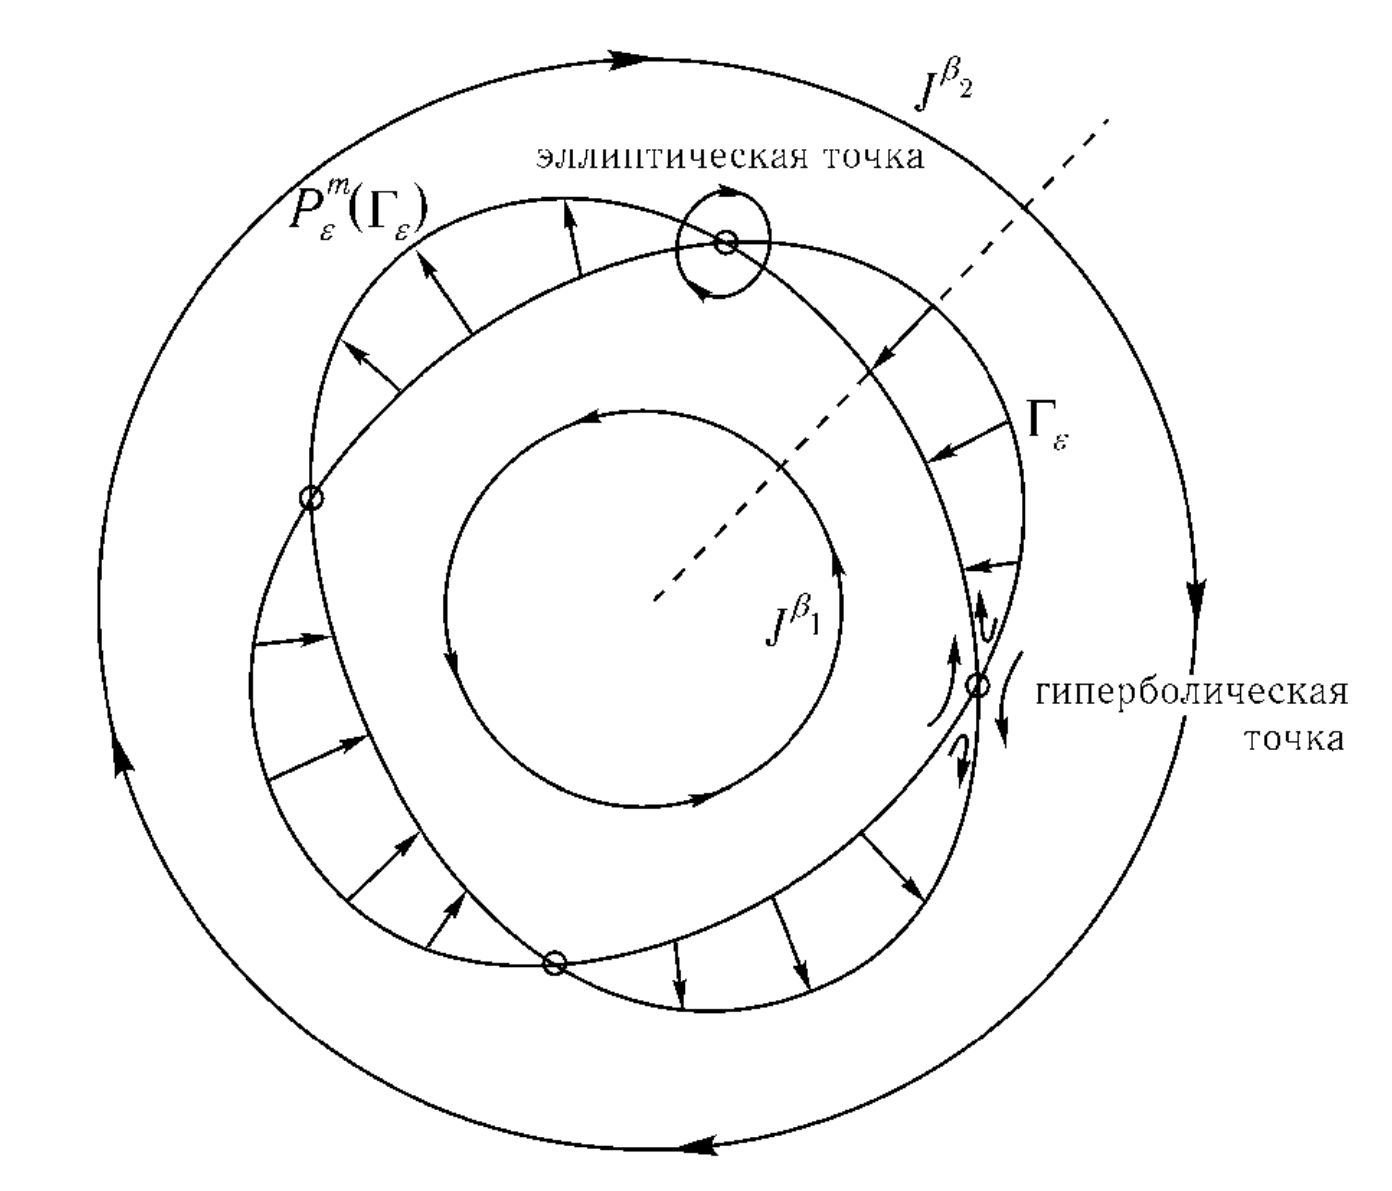
\includegraphics[width=0.5\textwidth]{pme}
\caption{Отображение $P^m_\varepsilon$, показывающее кривую $Gamma_\varepsilon$, ее образ $P^m_\varepsilon(\Gamma_\varepsilon)$ и неподвижные точки (по книге Арнольда и Авеца [1968]). Мы приводим рисунок по модулю $2\pi m$, поэтому кажется, что точки вращаются по часовой стрелке вне резонансной окружности и против часовой стрелки внутри нее.}
\label{fig:pic2}
\end{figure}

Далее, отображение сохраняет площади, поэтому кривые $Gamma_\varepsilon$ и $P^m_\varepsilon(\Gamma_\varepsilon)$ ограничивают одинаковые площади и, очевидно, должны пересекаться. Каждая точка пересечения является неподвижной для возмущенного отображения $P^m_\varepsilon$. Пуанкаре [1899] доказал существование $2km$, таких точек, где $k$ — некоторое (неизвестное) целое число: см. рисунок \ref{fig:pic2} (Ясно, что в типичном случае пересечения  $Gamma_\varepsilon$ и $P^m_\varepsilon(\Gamma_\varepsilon)$ трансверсальны и что общее их число должно быть четным и не менее $2m$.)

Типы устойчивости данных неподвижных точек можно определить из рассмотрения поведения близлежащих точек. Вначале заметим, что произведение собственных значений $\lambda_1, \lambda_2$ возмущенного отображения, линеаризованного в неподвижной точке, должно равняться единице, так как $\det{|DP^m_\varepsilon|} = 1$. Таким образом, вырожденные (параболические) точки с матрицей (\ref{eq:e4835}) перерождаются или в гиперболические неподвижные точки $0<\lambda_1<1<\lambda_2$, или в эллиптические неподвижные точки $(\lambda_2=\overline{\lambda_1})$. Предположив, что пересечения $Gamma_\varepsilon$ c $P^m_\varepsilon(\Gamma_\varepsilon)$ трансверсальны, легко увидеть из рисунка \ref{fig:pic2}, что ровно половина из них является эллиптическими центрами, а половина --- гиперболическими седлами, так как точки либо циркулируют вокруг неподвижной точки, либо <<монотонно>> покидают ее окрестность (см. Arnold, Avez [1968], \S 20).

\task{
Докажите последнее утверждение, полагая $P^m_\varepsilon$ равным
отображению за время 1 потока некоторого двумерного векторного поля и пользуясь
теорией индексов (ср. раздел 1.8).
} 

Инвариантные многообразия седел располагаются, очевидно, в промежутке между соседними «иррациональными» инвариантными кривыми, сохраняющимися для $P_\varepsilon$, и эти инвариантные многообразия обязаны пересекаться (в противном случае отображение не могло бы сохранять площади). В общем случае, некоторые из этих пересечений будут трансверсальными. Таким образом, в каждом <<резонансном поясе>> вблизи невозмущенной
кривой $J^\alpha$ можно ожидать существования некоторого сложного множества инвариантных кривых, подобных тем, которые мы попытались изобразить на рис. \ref{fig:pic3}. Zehnder~[1973] установил данный результат в типичном случае. Такие области в физической литературе называют \emph{стохастическими слоями}, а иногда --- \emph{гомоклиническими сплетениями}. Как мы увидим в главе 5, каждой точке трансверсального гомоклинического пересечения соответствует очередное счетное семейство гиперболических периодических точек, так что динамика в стохастическом слое очень сложна.
\begin{figure}
\centering
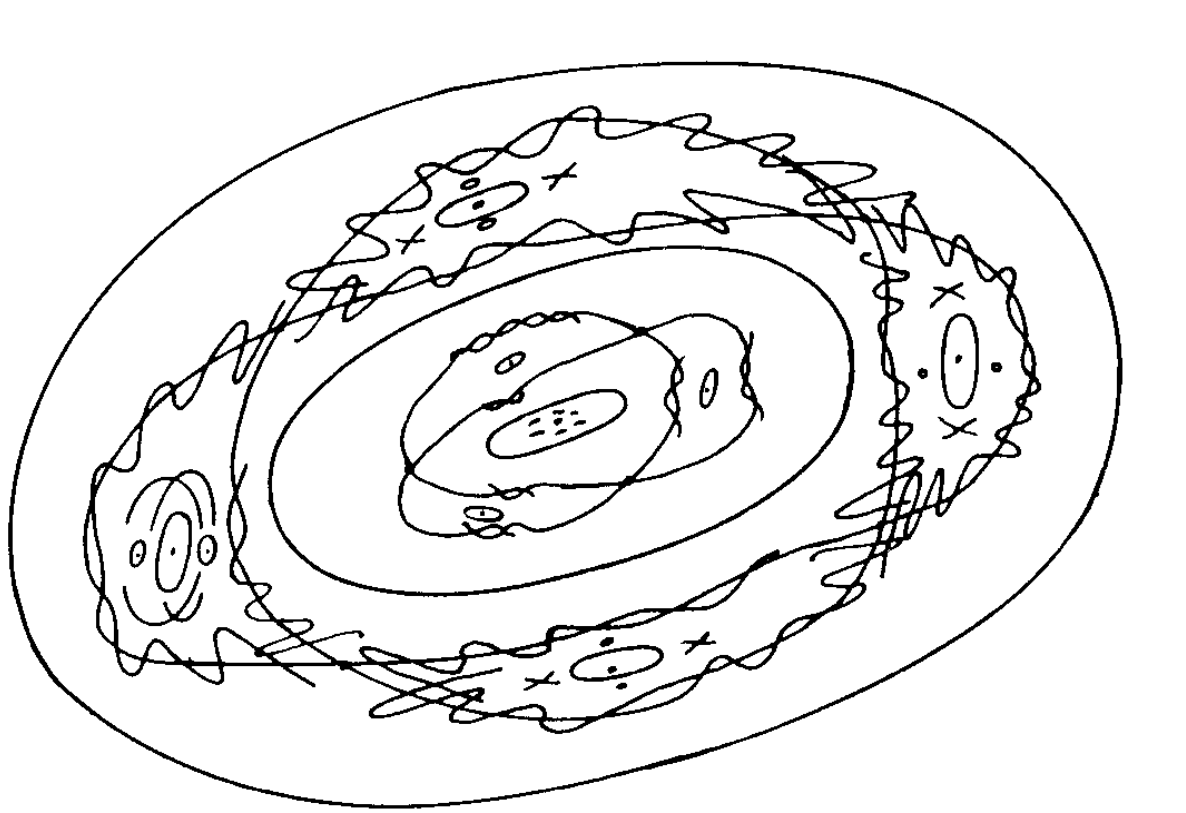
\includegraphics[width=0.5\textwidth]{curves}
\caption{Резонансные кривые в общем случае распадаются на стохастические слои}
\label{fig:pic3}
\end{figure}
\task{
В обсуждаемом контексте рассмотрите сохраняющее площадь отображение \\  \hbox{$f\colon (\phi, u) \to (\phi + u, u - \gamma \cos (\phi + u))$} из раздела 2.4 для малых значений $\gamma$. Найдите путем непосредственных расчетов какие-либо орбиты периода 2 (возможно, 3) и сравните их с гиперболическими и эллиптическими орбитами, появления которых можно ожидать при бифуркации подходящих резонансных замкнутых кривых. (См. Green [1980], где проводится массированная атака на эту проблему.)
}

Прорезюмированные выше результаты основывались на неконструктивных аргументах, позволяющих сделать вывод о трансверсальности пересечений. В противоположность этому, мы покажем в заключение данного раздела и главы, как можно использовать метод Мельникова для расчёта истинного поведения резонансных поясов в конкретных примерах.
Churchill [1982] одним из первых предложил такой подход. Вернемся к уравнению (\ref{eq:label3}), зафиксируем полную энергию $h$ и выберем $l^\alpha$ так, чтобы периодическая орбита $q^\alpha(\theta),  q^\alpha(\theta)$ невозмущенной системы
\begin{equation}
q' = -\frac{\partial L^0}{\partial p}, p'=-\frac{\partial L^0}{\partial q}
\end{equation}
имела период $T=2 \pi m/n$ по $\theta$ и, таким образом, резонанса $2 \pi$-периодическому возмущению $L^1$. Непосредственное применение метода Мельникова (теорема \ref{moserTheorem} и разделы 4.6-4.7) при учете того, что отображение Пуанкаре сохраняет площадь, приводит к следующему результату (доказательство оставляем читателю в качестве упражнения):
\mytheorem{
 Если субгармоническая функция Мельникова 
 \begin{equation}
M^{m/n}(\theta^0)=\int_0^{2 \pi m} \{L^0(q^\alpha(\theta),p^\alpha(\theta);h),L^1(q^\alpha(\theta),p^\alpha(\theta), \theta + \theta^0;h)\}\,d\theta
\label{eq:e4837}
\end{equation}
 не зависит от $\varepsilon$ и имеет $j$ простых корней на промежутке   $\theta^0 \in [0;2\pi m/n]$   , то резонансная замкнутая кривая $L^0 = l^\alpha$ для невозмущенного отображения Пуанкаре $P_0$ распадается на некоторое множество из $2k=j/m$ периодических орбит периода $m$. Кроме того, число $j$ необходимо является четным кратным $m$, и ровно $k$ периодических орбит гиперболичны и $k$-эллиптичны.
}\label{th3}

Как и в формулах (4.5.12)-(4.5.13), $\{L^0,L^1\}=(\partial L^0/\delta q)(\partial L^1/ \partial p) - (\partial L^0/\partial p)(\partial L^1 / \partial q)$ представляет собой скобку Пуассона функций $L^0$ и $L^1$. В конкретных примерах расчеты $L^0$ и $L^1$ по формулам (\ref{eq:label2}) зачастую слишком громоздки, и более удобно сформулировать теорему в терминах исходного гамильтониана $H^\varepsilon=F+G+\varepsilon H^1$. Непосредственные вычисления (с учетом (\ref{eq:label2})) дают
\begin{equation}
\{L^0,L^1\} = \frac{1}{\Omega^2(L^0)}\{F, H^1\},
\end{equation}

где $\{F, H^1\}(\partial F/\delta q)(\partial H^1/ \partial p) - (\partial F/\partial p)(\partial H^1 / \partial q)$ . Таким образом, используя тот факт, что на невозмущенном решении $q^\alpha, p^\alpha$ выполняется соотношение $\theta = \Omega(L^0(q^\alpha,p\alpha;h))t+\theta^0=\Omega(l^\alpha)t+\theta^0$, мы можем заменить (\ref{eq:e4837}) на
 \begin{equation}
 M^{m/n}(\theta^0)=\frac{1}{\Omega (l^\alpha)} \int_0^{2\pi m/\Omega (l^\alpha)} \{F(q^\alpha(t),p^\alpha(t)),H^1(q^\alpha(t),p^\alpha(t),\Omega(l^\alpha)t+\theta^0; l^\alpha)\}\,dt.
\end{equation}

\mytheorem{
Рассмотрим гамильтонову систему с двумя степенями свободы вида (\ref{eq:label1}) и допустим, что $F$ содержит гомоклиническую орбиту $(q^0(t),p^0(t)$, соединяющую некоторую гиперболическую седловую точку саму с собой (т.е. $P$ обладает гомоклиническим циклом). Предположим, что $\Omega(I)=G'(I)>0$ при $I>0$. Пусть $h^0 = F(q^0,p^0)$ --- энергия гомоклинической орбиты, а $h>h^0$ и $l_0=G^{-1}$ --- константы. Пусть $\{F,H^1\}(t+\theta^0)$ обозначает скобку Пуассона функций $F(q^0,p^0)$ и $H^1(q^0,p^0,\Omega(l^0)t+\theta^0;l^0$, вычисленную при $q=q^0(t)$ и $p=p^0(t)$.  Определим
\begin{equation}
M(\theta^0)= \int_{-\infty}^{\infty} \{F,H^1\}(t+\theta^0)\,dt,
\end{equation}
 и допустим, что $M(\theta^0)$ имеет простой нуль и не зависит от $\varepsilon$. Тогда для достаточно малых значений $\varepsilon > 0$ гамильтонова система, соответствующая (\ref{eq:label1}) имеет трансверсальные гомоклинические орбиты на энергетической поверхности $H^\varepsilon = h$
}\label{th4}

Из анализа трансверсальных гомоклинических орбит и обсуждения
подковы, предстоящих в главе 5, следует такое утверждение:

\mytheorem{Данная система обладает гиперболическим инвариантным множеством (см. ниже раздел 5.2) $\Lambda$ на энергетической поверхности $H=h$; $\Lambda$ обладает плотной орбитой, поэтому система не имеет второго глобального аналитического интеграла.
}
(Ziglin [1982] недавно опубликовал аналогичный результат.)

Если предположения теорем \ref{th3} и \ref{th4} выполнены, то невозмущенное и возмущенное отображения $P_0$ и $P_\varepsilon$ (см. (\ref{eq:e4826})-(\ref{eq:e4827})) обладают
структурами инвариантных кривых, изображенными на рисунке \ref{fig:pic4}.

\begin{figure}
\centering
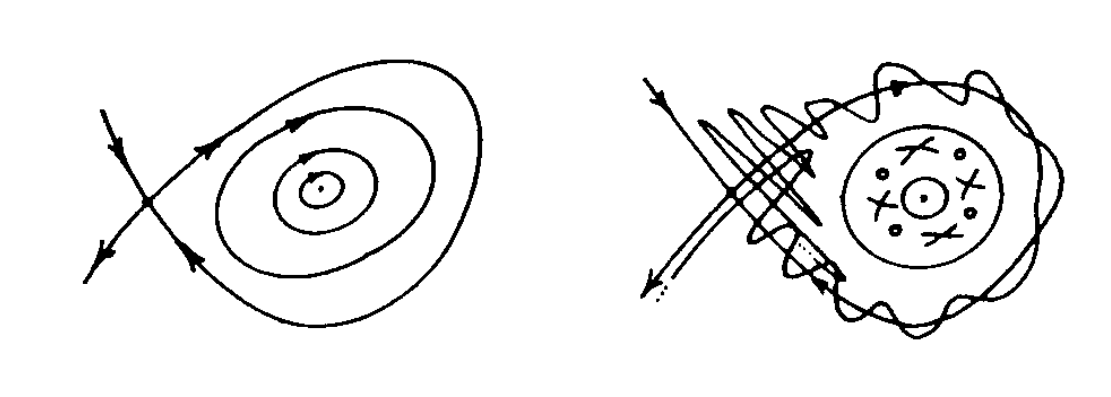
\includegraphics[width=0.5\textwidth]{pic4}
\caption{Инвариантные кривые невозмущенного и возмущенного отображений Пуанкаре: $(a) P_0;(b) P_\varepsilon$}
\label{fig:pic4}
\end{figure}

В качестве примера рассмотрим систему слабо связанных маятника и линейного осциллятора (см. Holmes, Marsden [1982а]) с гамильтонианом 
\begin{equation}
H^\varepsilon(p,q,x,y) = \frac{p^2}{2}+(1-\cos q)+\frac{y^2+\omega^2x^2}{2}+\varepsilon \frac{(x-q)^2}{2},
\label{eq:e4841}
\end{equation}
(см. упражнение \ref{osc}). Перейдем от системы $x,y$ к переменным
<<действие-угол>> по формулам
$$x = \sqrt{\frac{2I}{\omega}}\sin \theta, \text{~~} I=\sqrt{2\omega I}\cos \theta$$
тогда функция (\ref{eq:e4841}) примет вид
\begin{equation}
H^\varepsilon = \frac{p^2}{2}+(1-\cos q)+\omega I+\frac{\varepsilon}{2}\left(\sqrt{\frac{2I}{\omega}}\sin \theta - q\right)^2=F(q,p)+G(I)+\varepsilon H^1(q,p,I,\theta).
\label{e4842}
\end{equation}

Система $F$ имеет пару гомоклинических орбит
\begin{equation}
(q^0(t),p^0(t))=(\pm2\arctg (\sh(t)),\pm2\sech y)
\end{equation}
с энергией
\begin{equation}
F(q,p)=h^0=2
\end{equation}

Следовательно, мы возьмем $h>2$ и положим
\begin{equation}
l^0=G^{-1}(h-h^0)=\frac{1}{\omega}(h-2)
\end{equation}

Теперь можно оценить функцию Мельникова, пользуясь формулой
\begin{equation}
\{F,H^1\}=\frac{\partial F}{\partial q}\frac{\partial H^1}{\partial p}-\frac{\partial F}{\partial p}\frac{\partial H^1}{\partial q} =p\left(\sqrt{\frac{2I}{\omega}}\sin \theta -q\right),
\end{equation}
тде скобки Пуассона надо вычислять на орбите $(q^0(t),p^0(t),\theta(t)=\omega t + \theta^0, I(t)=l^0)\colon$
\begin{equation}
M(\theta^0)=\int_{-\infty}^{\infty}2\sech(t)\left(-2\arctg(\sh t)\pm\frac{\sqrt{2(h-2)}}{\omega}\sin(\omega t + \theta^0)\right)
\label{e4847}
\end{equation}
Здесь <<плюс>> относится к верхней ветви гомоклинической орбиты $(p > 0)$, а <<минус>> — к нижней $(p < 0)$. Первый интегрант в формуле (\ref{e4847}) нечетен, и интеграл от него равен нулю, второй интегрант можно оценить методом вычетов; в результате получим
\begin{equation}
M(\theta^0)=\pm\frac{2\pi\sqrt{2(h-2)}}{\omega}\sech\left(\frac{\pi\omega}{2}\right)\sin\theta^0
\end{equation}
Поскольку функция $M(\theta^0)$ имеет простые корни, условия теоремы \ref{th4} выполнены, и мы можем сделать вывод, что возмущенная (связанная) система имеет трансверсальные гомоклинические орбиты и, следовательно,
подковы Смейла на каждом уровне энергии $h>2$ для достаточно малых (зависящих от $h$) значений $\varepsilon$.

\task{
Выясните судьбу резонансных торов для гамильтониана (\ref{e4842}), заданных значениями $F(q,p)=h^\alpha<2$ и $I=l^0=(1/\omega)(h-h^\alpha)>0$
} 
\task{
Рассмотрите возмущение гамильтониана типа Hénon-Helies
$$H(\dot x,\dot y,x,y)=\frac{\dot x^2+\dot y^2}{2}+\frac{\omega^2(x^2+y^2}{2}-x^2y-\frac{y^3}{3}+\varepsilon(\alpha y^2-\beta y^3),$$
$$0\leq\varepsilon\ll1; \text{~~} \alpha,\beta=O(1).$$
}

Докажите, что эта система интегрирусма при $\varepsilon = 0$ и неинтегрируема при малых $\varepsilon \neq 0$. (Подсказка: воспользуйтесь симплектическим преобразованием
$$\begin{array}{cc}
q_1=\frac{1}{\sqrt{2}}(x+y) & q_1=\frac{1}{\sqrt{2}}(x-y)\\
p_1=\frac{1}{\sqrt{2}}(\dot x+\dot y) & q_1=\frac{1}{\sqrt{2}}(\dot x-\dot y)
\end{array}$$

См. Holmes [1982b] и упражнение 1.8.14.)

Заметим, что теорию двумерных сохраняющих площаль отображений, обсуждавшуюся в данном разделе, можно непосредственно применять к гамильтоновым системам с периодическим возмущением вида
\begin{equation}
H^\varepsilon(q,p,t)=F(q,p)+\varepsilon H^1(q,p,t).
\end{equation}

Уравнение Дуффинга, рассматривавшееся в разделах 4.5-4.6, принимает такую форму, когда коэффициент вязкого трения $\delta$ полагается равным нулю. Уменьшая $\delta$ при фиксированных $\gamma, \omega >0$, мы приближаемся к гамильтонову пределу, а соответствующие бифуркации (см. рисунок 4.6.3), в результате
которых создаются счетные множества периодических и гомоклинических орбит, следует рассматривать как ступени в создании гомоклинического сплетения и стохастических слоев, изображенных на рисунке \ref{fig:pic3}.

В заключение отметим, что теоремы \ref{th3}-\ref{th4} имеют многомерные аналоги, относящиеся к гамильтоновым системам с $n$ степенями свободы (см. Holmes, Marsden[1982a,b]), и что Gruendler [1982, 1985] получил также многомерное обобщение теории Мельникова. В действительности, в определенных случаях теория Мельникова применима к исследованию возмущений бесконечномерных гамильтоновых эволюционных уравнений, возникающих из уравнений в частных производных.  Holmes, Marsden [1981] провели анализ некоторых таких ситуаций с примером из механики, являющимся, по существу, бесконечномерным обобщением уравнения Дуффинга, описывающего вынужденные демпфированные колебания непрерывной балки, подверженной продольной нагрузке, рассмотренные в разделе 2.2. Кроме того, Holmes [1981b] применил эти методы к уравнению в частных
производных типа синус Гордона
$$\phi_{tt}-\phi_{xx}+\sin\phi=-\varepsilon\phi_t$$
с зависящими от времени граничными условиями
$$\phi_x(0,t)=\varepsilon H,$$
$$\phi_x(1,t)= \varepsilon (H+I(t)).$$
\end{document}

